\section{Extending the \dcel\label{arr_sec:ex_dcel}}
%============================

For many applications of the arrangement package it is necessary to
store additional information (perhaps of non-geometric nature) with
the arrangement cells. As vertices are associated with \ccc{Point_2}
objects and edges (halfedge pairs) are associated with
\ccc{X_monotone_curve_2} objects, both defined by the traits class,
it is possible to extend the traits-class type by using a traits-class
decorator, as explained in Section~\ref{arr_ssec:meta_tr}, which may
be a sufficient solution for some applications.
However, the \dcel\ faces are not associated with any geometric object, 
so it is impossible to extend them using a traits-class decorator. 
Extending the \dcel\ face records comes handy is such cases. As a matter
of fact, it is possible to conveniently extend all \dcel\ records
(namely vertices, halfedges and faces), which can also be advantageous
for some applications.

All examples presented so far use the default \ccc{Arr_default_dcel<Traits>}. 
This is done implicitly, as this class serves as a default parameter for 
the \ccc{Arrangement_2} template. The default \dcel\ class just associates 
points with vertices and $x$-monotone curves with halfedge, but nothing more. 
In this section we show how to use alternative \dcel\ types to extend the 
desired \dcel\ records.

\subsection{Extending the \dcel\ Faces\label{arr_ssec:ex_dcel_face}}
%--------------------------------------

The \ccc{Arr_face_extended_dcel<Traits, FaceData>} class-template
is used to associate auxiliary data field of type \ccc{FaceData} to
each face record in the \dcel.

When an \ccc{Arrangement_2} object is parameterized by this 
\dcel\ class, its nested \ccc{Face} type is extended with the access function
\ccc{data()} and with the modifier \ccc{set_data()}. Using these extra
functions it is straightforward to access and maintain the auxiliary
face-data field.

Note that the extra data fields must be maintained by the application
programmers. They may choose to construct their arrangement, and
only then go over the faces and attach the appropriate data fields to
the arrangement faces. However, in some cases the face data can only
be computed when the face is created (split from another face, or merged
with another face). In such cases one can use an arrangement observer
tailored for this task, which receives updates whenever a face is
modified and sets its data field accordingly.

\begin{figure}[t]
\begin{ccTexOnly}
  \begin{center}
  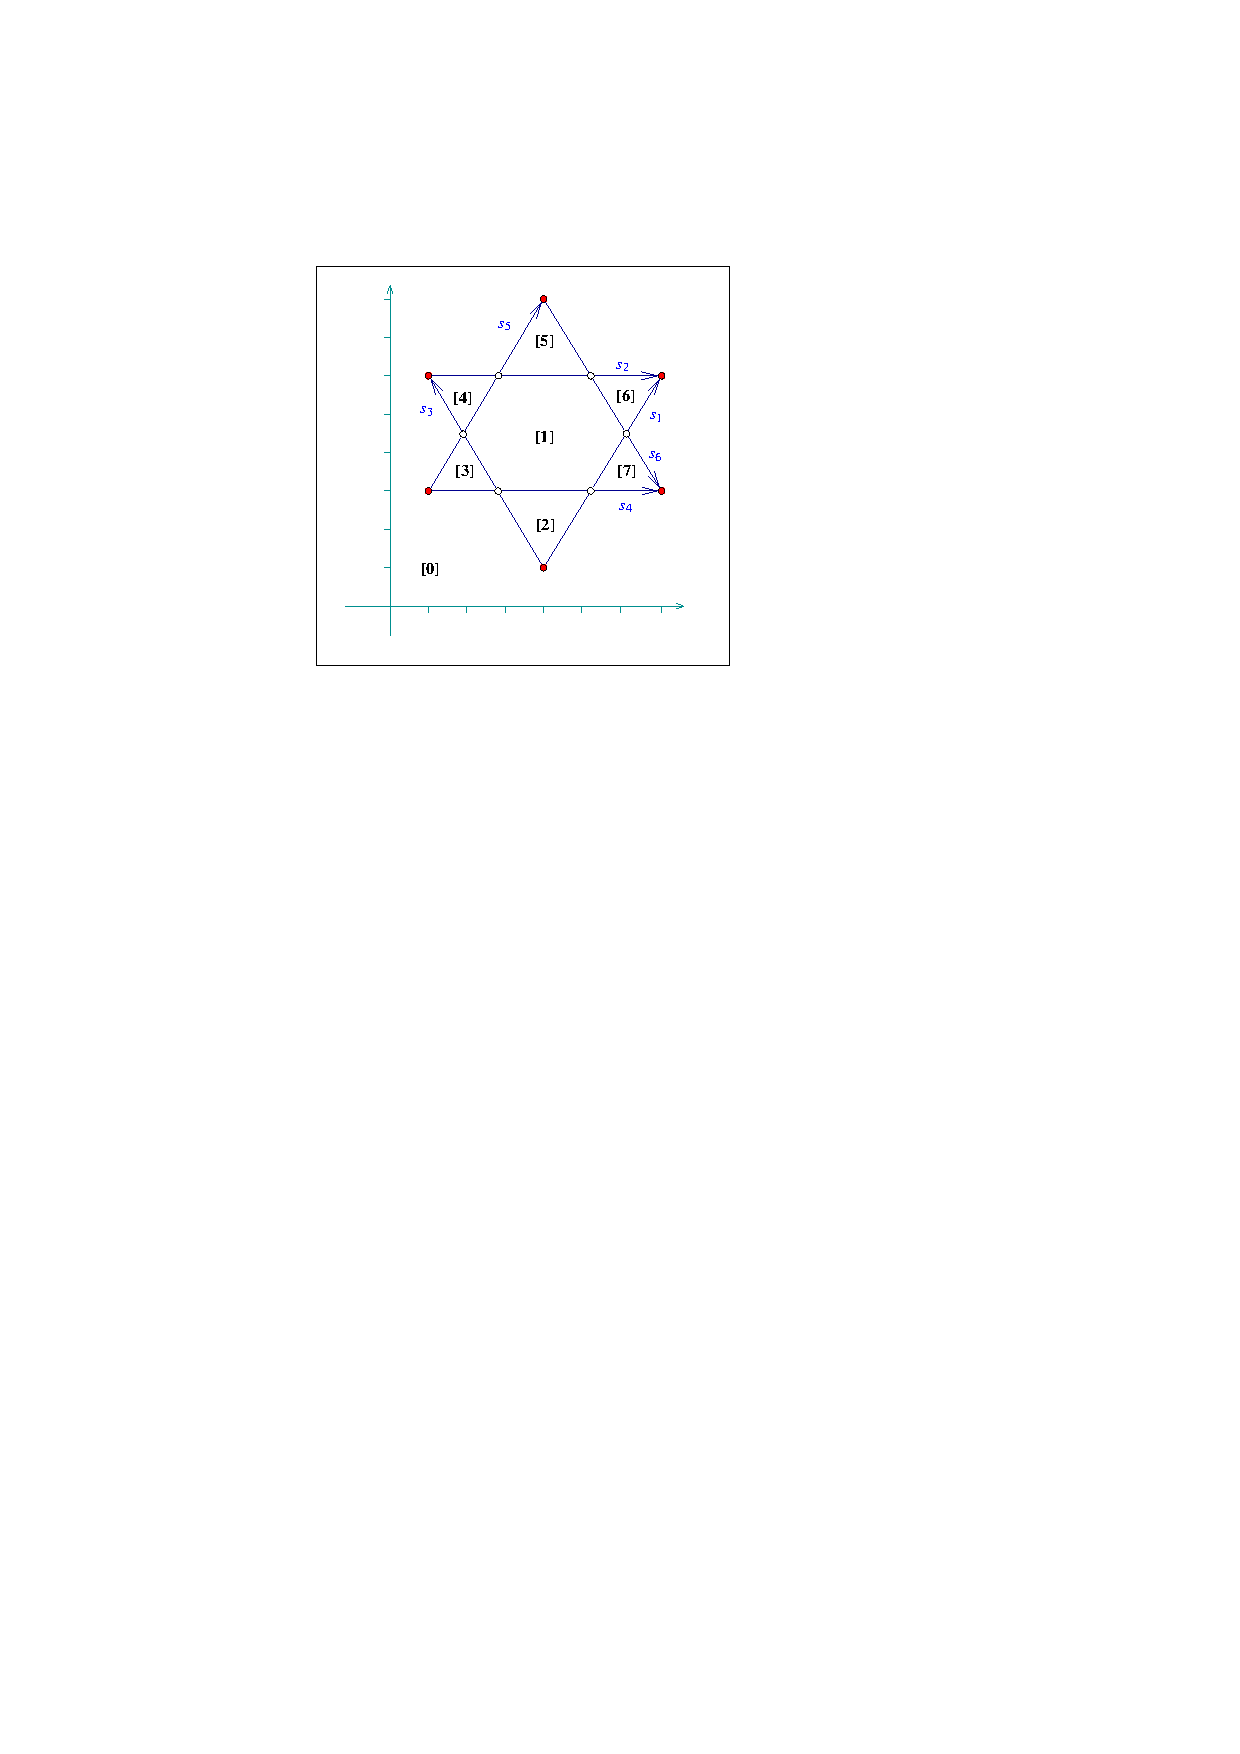
\includegraphics{Arrangement_2/fig/ex_20}
  \end{center}
\end{ccTexOnly}
\begin{ccHtmlOnly}
  <p><center>
  <img src="./fig/ex_20.gif" border=0 alt="Example 20">
  </center>
\end{ccHtmlOnly}
\caption{An arrangement of six line segments, as constructed in
\ccc{face_extension.cpp} and \ccc{dcel_extension.cpp}
(in \ccc{dcel_extension.cpp} we treat
the segments as directed, so they are drawn as arrows directed from the
source to the target). The indices associated with the halfedges in
\ccc{face_extension.cpp} are shown in brackets.\label{arr_fig:ex_20}}
\end{figure}

The next example constructs an arrangement that contains seven bounded 
faces induced by six line segments (see Figure~\ref{arr_fig:ex_20}). An 
observer gets notified each time a new face $f$ is created and it associates 
$f$ with a running index, (where the index of the unbounded face
is 0). As a result, the faces are numbered according to their creation
order, as one can easily verify by examining the insertion order of the
segments:\footnote{For simplicity, the particular observer used must be
attached to an empty arrangement. It is not difficult however to modify 
the program to handle the general case of attaching a similar observer
to a non-empty arrangement.}

\ccIncludeExampleCode{Arrangement_2/face_extension.cpp}

\subsection{Extending All \dcel\ Records\label{arr_ssec:ex_dcel_all}}
%----------------------------------------

The \ccc{Arr_extended_dcel<Traits, VertexData, HalfedgeData, FaceData>}
class-template is used to associate auxiliary data fields of
types \ccc{VertexData} \ccc{HalfedgeData}, and \ccc{FaceData} to
each \dcel\ vertex, halfedge, and face record types, respectively.

When an \ccc{Arrangement_2} object is injected with this
\dcel\ class, each one of its nested \ccc{Vertex}, \ccc{Halfedge} and
\ccc{Face} classes is extended by the access function \ccc{data()}
and by the modifier \ccc{set_data()}.

The next example shows how to use a \dcel\ with extended vertex,
halfedge, and face records. In this example each vertex is associated 
with a color, which may be blue, red, or white, depending on whether the
vertex is isolated, represents a segment endpoint, or whether it
represents an intersection point. Each halfedge is associated with
Boolean flag indicating whether its direction is the same as the
direction of its associated segment (in this example segments are
treated as directed objects). Each face is also extended to store the
size of its outer boundary.

The constructed arrangement, depicted in Figure~\ref{arr_fig:ex_20}, is 
similar to the arrangement constructed in the previous example. 
Note that all auxiliary data fields are set during the construction phase.
Also note that the data fields are properly maintained when the arrangement
is copied to another arrangement instance:
 
\ccIncludeExampleCode{Arrangement_2/dcel_extension.cpp}

\begin{ccAdvanced}
The various \dcel\ classes presented in this section are perfectly
sufficient for most applications based on the arrangement package.
However, users may also use their own implementation of a \dcel\ class
to instantiate the \ccc{Arrangement_2} class-template, in case they need
special functionality from their \dcel. Such a class must be a model of the
concept \ccc{ArrangementDcel}, whose exact specification is listed in the
Reference Manual.
\end{ccAdvanced}
